%\documentclass[iop]{emulateapj}
%\documentclass[12pt, preprint]{emulateapj}
\documentclass[12pt, onecolumn]{emulateapj}

\usepackage{tikz}
\usetikzlibrary{shapes.geometric, arrows}
\usetikzlibrary{fit}

\tikzstyle{hyper} = [rectangle, rounded corners, minimum width=1cm, minimum height=0.5cm,text centered, draw=black, fill=blue!30]
\tikzstyle{param} = [rectangle, rounded corners, minimum width=1cm, minimum height=0.5cm,text centered, draw=black, fill=green!30]
\tikzstyle{data} = [rectangle, rounded corners, minimum width=1cm, minimum height=0.5cm,text centered, draw=black, fill=red!30]
%\tikzstyle{hyper} = [trapezium, trapezium left angle=70, trapezium right angle=110, minimum width=1cm, minimum height=0.5cm, text centered, draw=black, fill=green!30]
%\tikzstyle{param} = [rectangle, minimum width=1cm, minimum height=0.5cm, text centered, draw=black, fill=green!30]
%\tikzstyle{data} = [diamond, minimum width=1cm, minimum height=1cm, text centered, draw=black, fill=red!30]
\tikzstyle{eqn} = [rectangle, minimum width=1cm, minimum height=0.5cm, text centered, draw=black]%, fill=green!30]
\tikzstyle{latent} = [diamond, minimum width=1cm, minimum height=0.5cm, text centered, draw=black]%, fill=green!30]
\tikzstyle{arrow} = [thick,->,>=stealth]

\newcommand{\myemail}{aimalz@nyu.edu}
\newcommand{\textul}{\underline}

\shorttitle{Probabilistic Redshift Distribution}
\shortauthors{Malz}

\begin{document}

\title{Probabilistic Redshift Distribution: Minimal Approach}

\author{A.I. Malz\altaffilmark{1}}
\altaffiltext{1}{CCPP}
\email{aimalz@nyu.edu}

\begin{abstract}
This paper outlines a method for calculating the redshift distribution function $N(z)$ from a set of posteriors for the photometric redshifts of individual galaxies.
\end{abstract}

\keywords{photo-z}

\section{Introduction}

The redshift distribution function $N(z)$ indicates the expected number of galaxies at each redshift.  

\section{Method}

\subsection{Probabilistic Model}

We would like to learn the redshift distribution function $N(z)$ describing the number of galaxies at each redshift.  Redshifts are parameters we would like to estimate, and the parameters $N$ determining $N(z)$ may be considered hyperparameters that determine the probability of a redshift occurring.  The redshift distribution function may be expressed as Eq. \ref{eq:params}.

\begin{eqnarray}
\label{eq:params}
p(z|N) &=& \frac{N(z)}{\int N(z)\ dz} = \frac{N(z)}{E[N]}
\end{eqnarray}

Let us consider a galaxy $j$ whose data $\vec{d}_{j}$ is a set of magnitudes in each of several filters and seek the likelihood of observing the data under the model $N(z)$.  We may express this likelihood $p(\vec{d}_{j}|N)$ in terms of the likelihood $p(\vec{d}_{j}|z)$ as in Eq. \ref{eq:likelihood}.  However, it is generally considered impossible to calculate $p(\vec{d}_{j}|z)$ from $\vec{d}_{j}$.  It is easy to find the posterior probability $p(\vec{d}_{j}|z,N_{0})$ of a galaxy's photometry given its redshift and an assumed redshift distribution function $N_{0}(z)$ serving as an uninformative prior.  This has been done by \citet{she11}, for example.  We may use this posterior to find the likelihood function $p(\vec{d}_{j}|N)$ for the observed data $\vec{d}_{j}$ under an arbitrary redshift distribution function $N(z)$, as in Eq. \ref{eq:posterior}.  \citep{mar15}

\begin{eqnarray}
\label{eq:likelihood}
p(\vec{d}_{j}|N) &=& \int\ p(\vec{d}_{j}|z)\ p(z|N)\ dz\\
&=& \int\ p(\vec{d}_{j}|z)\ p(z|N)\ \frac{p(z|\vec{d}_{j},N_{0})}{p(z|\vec{d}_{j},N_{0})}\ dz\nonumber\\
&=&  \int\ p(\vec{d}_{j}|z)\ p(z|N)\ \frac{p(z|\vec{d}_{j},N_{0})\ p(\vec{d}_{j}|N_{0})}{p(\vec{d}_{j}|z)\ p(z|N_{0})}\ dz\nonumber\\
\label{eq:posterior}
&=& \int\ p(z|N)\ p(z|\vec{d}_{j},N_{0})\ \frac{p(\vec{d}_{j}|N_{0})}{p(z|N_{0})}\ dz\nonumber\\
&\propto& \int\ p(z|\vec{d}_{j},N_{0})\ \frac{p(z|N)}{p(z|N_{0})}\ dz
%\prod_{j=1}^{J}\ p(\vec{d}_{j})\ \int p(z|N)\ \frac{p(z|\vec{d}_{j})}{p(z)}\ dz
\end{eqnarray}

Now let us consider an ensemble of $J$ galaxies.  The full dataset of $\{\vec{d}_{j}\}_{j=1,\dots,J}$ will be denoted as $\textul{D}$.  The likelihood function for the redshift distribution function is given in Eq. \ref{eq:fulllikelihood}, where the likelihoods for each galaxy's redshift are assumed to be independent.  

\begin{eqnarray}
\label{eq:fulllikelihood}
p(\textul{D}|N) &=& \prod_{j=1}^{J}\ p(\vec{d}_{j}|N)
\end{eqnarray}

Here, we would also like to calculate the posterior $p(N|\textul{D})$ for direct comparison with prior work in the literature.  The posterior may be calculated via Eq. \ref{eq:bayes} in terms of the prior distribution $p(N)$.  Since we cannot know $p(\textul{D})$, we sample the desired distribution using Monte Carlo-Markov chain (MCMC) methods.  

\begin{eqnarray}
\label{eq:bayes}
p(N|\textul{D}) &=& \frac{p(\textul{D}|N)p(N)}{p(\textul{D})}
\end{eqnarray}

\subsection{Fake Data}
\label{sec:fake}

We consider the $K=35$ redshift bins $B_{k}=[z^{B}_{k-1},z^{B}_{k}]$ for which \citet{she11} calculated posteriors for the redshift of each galaxy based on observations of the apparent magnitude in the five photmetric filters of SDSS.  We shall take $\vec{\theta}$ to be a discretized parametrization of $N(z)$, where $\theta_{k}$ is the average value of $N(z)$ over the redshift range of bin $B_{k}$.   Thus the expected number of galaxies in each bin is $J_{k}=\theta_{k}\Delta_{k}$, where $\Delta_{k}\equiv z_{k+1}-z_{k}$, transforming Eq. \ref{eq:params} into Eq. \ref{eq:dparams} (although we actually work with the log of $\vec{\theta}$ throughout).  

\begin{eqnarray}
\label{eq:dparams}
p(B_{k}) &\equiv& \frac{J_{k}}{J} = \frac{\theta_{k}\Delta_{k}}{J}
%N(B_{k}) &=& \theta_{k} = J\tilde{\theta}_{k}\Delta_{k}% \frac{\mathcal{N}_{k}}{\sum_{k=1}^{K}\mathcal{N}_{k}}
\end{eqnarray}

In order to simulate data, we select set a true, physically motivated redshift probability distribution $p^{0}(z)$, where $p(z)$ corresponds to $N(z)$ for $J=1$.  The convolution of a linear function and a sum of Gaussians is quite general and accurately generates features observed in the true $N(z)$.  (Cite this!)  The instance of $p^{0}(z)$ here is shown in Eq. \ref{eq:truepz}, where the constant $C_{c}$ indicates the relative amplitude of the Gaussian component centered at $z_{c}$ with variance $\sigma_{c}^{2}$.  The linear function is evaluated at the centers of the bins $\bar{z}_{k}=(z_{k+1}-z_{k})/2$ and is included to ensure that $\lim_{z\to0}N(z)=0$.  The construction of this probability density is illustrated in Fig. \ref{fig:truepz}.  

\begin{eqnarray}
\label{eq:truepz}
p^{0}(z_{k}) &=& \sum_{c=1}^{6}\bar{z}_{k}C_{c}\int_{z_{k}}^{z_{k+1}} \mathcal{N}(z_{c},\sigma^{2}_{c})dz
\end{eqnarray}

\begin{figure}
\label{fig:truepz}
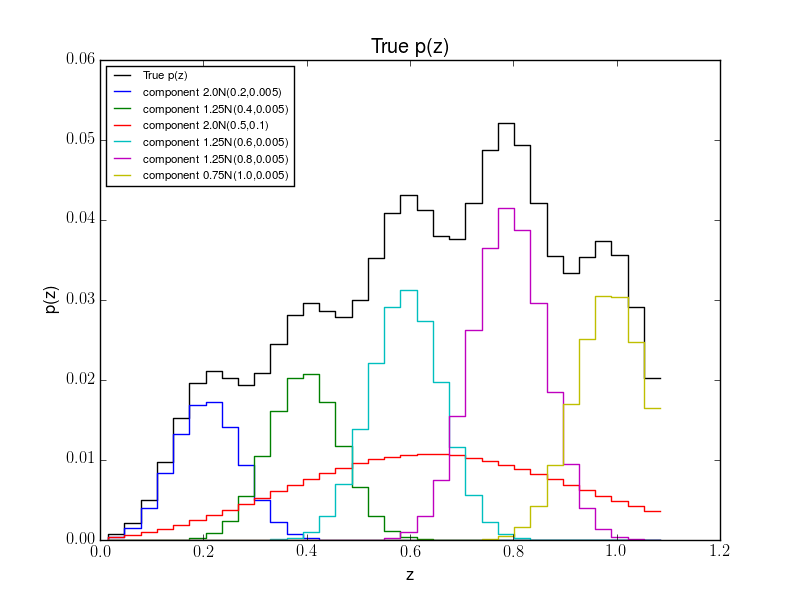
\includegraphics[scale=0.5]{truePz.png}
\caption{We construct $p^{0}$ as a sum of Gaussians.}
\end{figure}

We evaluate $p^{0}(z)$ over each bin to obtain $\vec{\theta}^{0}$ according to Eq. \ref{eq:truenz}, whose construction is illustrated in Fig. \ref{fig:truenz}.  The number of galaxies $J$ is selected from a Poisson distribution centered at an arbitrary $J_{0}=10,000$ galaxies.

\begin{eqnarray}
\label{eq:truenz}
\theta_{k} &\equiv& J\int_{z_{k}}^{z_{k+1}}p^{0}(z) dz
\end{eqnarray}

Next, we generate galaxy redshift likelihood functions as follows.  We first assign a bin number $b_{j}=k$ from $k=1,\dots,K$ to each galaxy $j$ by randomly sampling the $K$ bins with weights given by the true redshift function as $\int_{z_{k}}^{z_{k+1}}p^{0}(z)dz$.  Examples of some such samples for a fixed $J=1,000$ are shown in Fig. \ref{fig:obsnz}.

\begin{figure}
\label{fig:obsnz}
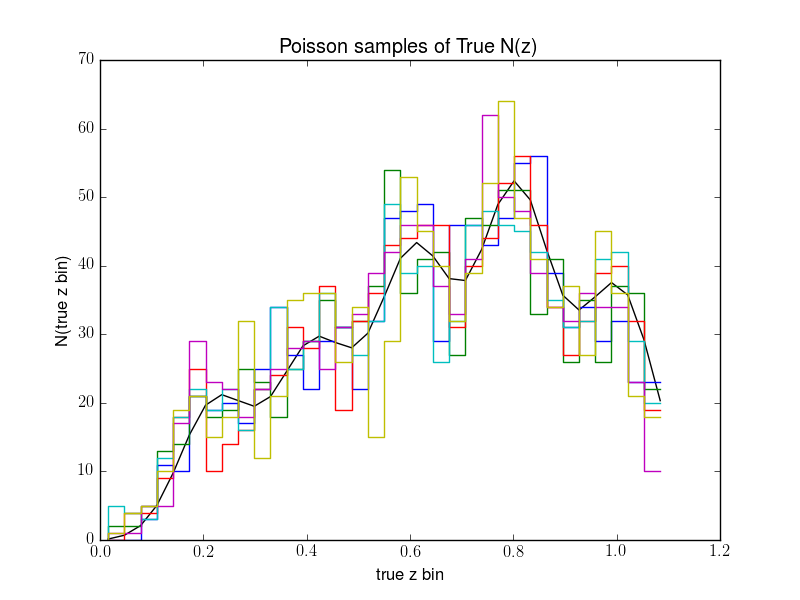
\includegraphics[scale=0.5]{obsNz.png}
\caption{Samples of the number of galaxies in each bin are generated as Poisson draws.}
\end{figure}

We then assign each galaxy a true redshift $z_{j}$ chosen uniformly from within the bin $B_{b_{j}}$ to which it was assigned.  The true redshift of each galaxy is shifted by a random error according to Eq. \ref{eq:zshift} to simulate inaccuracy in measurements, yielding a shifted redshift $z_{j}'$ for each galaxy.  Fig. \ref{fig:samples} shows histograms of the fake data generated.  It is worth noting that any method aiming to calculate the posterior should be unable to do better than the ``observed redshifts'' that go into generating the data.  SOMEHOW THIS IS NOT TRUE FOR THIS DATA, BUT HOW?

\begin{mathletters}
\begin{eqnarray}
\label{eq:zshift}
z_{j}' &=& z_{j}+e_{j}\\
p(e_{j}) &=& \mathcal{N}(0,\delta_{j})\nonumber\\
\delta_{j} &=& \frac{\sum_{b_{k}=1}^{K}(z_{b_{k}}-z_{b_{k}-1)}}{K}(1+z_{j})\nonumber
\end{eqnarray}
\end{mathletters}

\begin{figure}
\label{fig:samples}
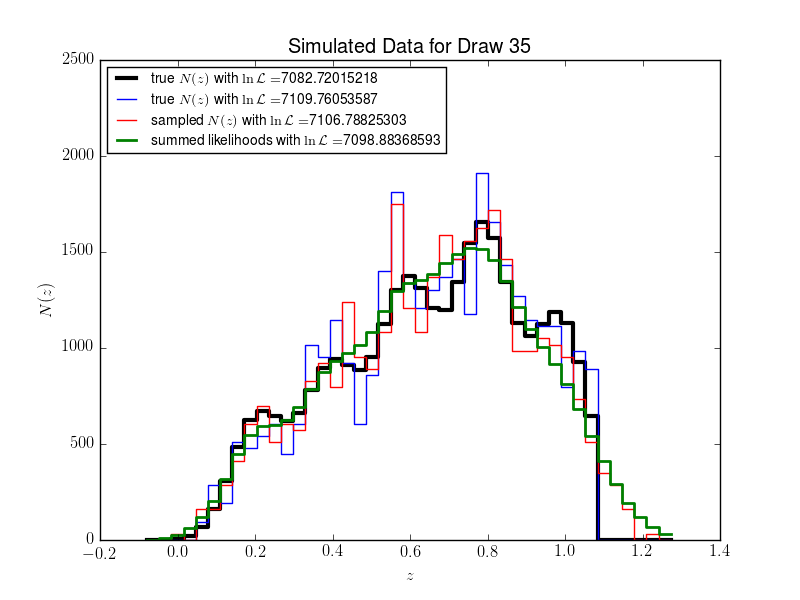
\includegraphics[scale=0.5]{exdata.png}
\caption{The true $\vec{\theta}$ chosen for this test is plotted here, along with histograms of the true redshifts sampled from it and the shifted redshifts resulting from the fake data generation procedure.}
\end{figure}

The discretized likelihood function $p(\vec{d}_{j}|B_{k})$ for each galaxy is taken to be Gaussian with a mean equal to the shifted redshift and a standard deviation proportional to $1+z_{j}$ to simulate the fact that uncertainty increases with redshift.  According to the above, "the data" are thus comprised of $J$ pairs $(z_{j}',\delta_{j})$.  The observed probability that galaxy $j$ has a redshift in bin $k$ is given by Eq. \ref{eq:zdist}.  As a final step, all likelihoods are normalized such that they integrate to unity over the redshift range spanned by the bins.  Fig. \ref{fig:pzs} shows a few examples of simulated likelihoods.

\begin{eqnarray}
\label{eq:zdist}
p(\vec{d_{j}}|B_{k}) = \int_{z_{k}}^{z_{k+1}} \frac{1}{\sqrt{2\pi\delta_{j}^{2}}}\exp\left[-\frac{(z_{j}'-z)^{2}}{2\delta_{j}^{2}}\right]\ dz
\end{eqnarray}

\begin{figure}
\label{fig:pzs}
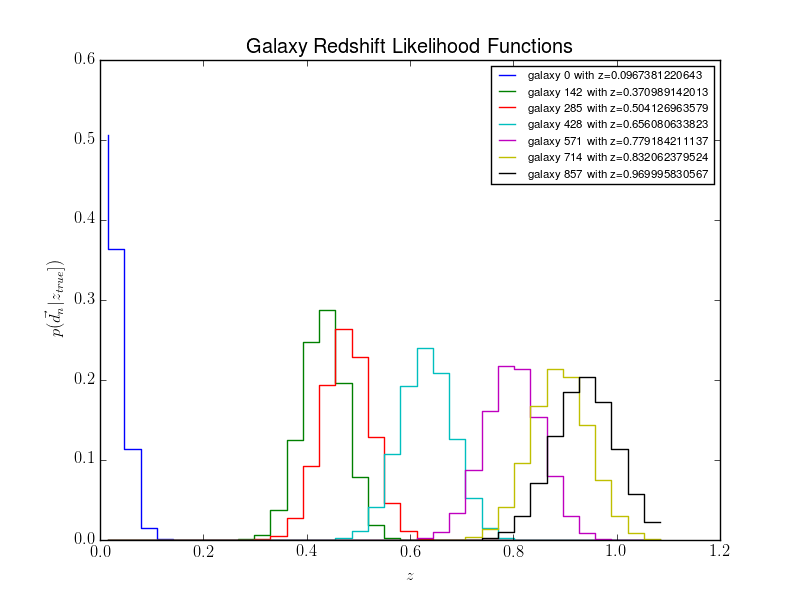
\includegraphics[scale=0.5]{lik-samps.png}
\caption{Several random redshift likelihood functions are shown here.  Note that the width of the Gaussian increases with redshift.}
\end{figure}

The likelihood function for the entire dataset given in Eq. \ref{eq:likelihood} may be re-expressed as Eq. \ref{eq:fulllik} in terms of $N(z)$ rather than $p(z)$.  It is valuable to verify that the likelihood is maximized for the true $N(z)$ that generated a particular set of simulated data.

\begin{eqnarray}
\label{eq:fulllik}
p(\textul{D}|N(z)) &=& \exp\left[-\int N(z)dz\right] \prod_{j=1}^{J}\int p(\vec{d}_{j}|z)N(z)dz\\
p(\textul{D}|\vec{\theta}) &=& \exp\left[-\sum_{k=1}^{K}\theta_{k}\Delta_{k}\right] \prod_{j=1}^{J}\sum_{k=1}^{K} p(\vec{d}_{j}|B_{k})\theta_{k}\Delta_{k} \nonumber\\
\ln p(\textul{D}|\vec{\theta}) &=& -\sum_{k=1}^{K}\exp\left[\ln\theta_{k}+\ln\Delta_{k}\right]+\sum_{j=1}^{J}\ln\left[\sum_{k=1}^{K}\exp\left[\ln p(\vec{d}_{j}|B_{k})+\ln\theta_{k}+\ln\Delta_{k}\right]\right] \nonumber
\end{eqnarray}

\section{Results}

The Metropolis-Hastings algorithm is applied to sample the posterior.  The procedure is initialized with the log of the average probability $\ln\theta^{0}_{k}=-\ln K\ \forall\ k$ (i.e. the flat distribution), which shall be denoted $\ln\vec{\theta}\equiv\ln p(z)$.  The log of the numerator of the posterior of Eq. \ref{eq:bayes} is calculated according to Eq. \ref{eq:disc-post} and is denoted as $\ln\tilde{p}(\vec{\theta}|\textul{D})$.  

\begin{eqnarray}
\label{eq:disc-post}
\ln\tilde{p}(\vec{\theta}'|\textul{D}) &\equiv& \ln p(\vec{\theta}') + \sum_{j=1}^{J}\ln\left[\sum_{k=1}^{K}p(\vec{d}_{j}|z_{k})\ p(z_{k}|\vec{\theta}')\right] \propto \ln p(\vec{\theta}'|\textul{D})\\
%\ln p(\vec{\theta})_{k} &=& \mathcal{N}(K^{-1},\textul{\Sigma})\nonumber\\
%\Sigma_{ij} &=& \left\{\begin{array}{cc}i=j&\ 1\\|i-j|=1&\ \frac{1}{2}\\else&0\end{array}\right\}
\end{eqnarray}

At each iteration $i$, proposal distribution $\vec{\theta}^{i}$ is generated from the multivariate normal distribution shown in Eq. \ref{eq:covmat}.  This covariance structure is chosen to enforce continuity of the histogram heights.  Some examples of samples from the initialization value are shown in Fig. \ref{fig:priors}.

\begin{mathletters}
\begin{eqnarray}
\label{eq:covmat}
\ln\vec{\theta}^{i} &=& \mathcal{N}(\ln\vec{\theta}^{i-1},\textul{\Sigma})\\
\Sigma_{kk'} &=& q\exp^{-\frac{a(k-k')^{2}}{2}}\nonumber
\end{eqnarray}
\end{mathletters}

\begin{figure}
\label{fig:priors}
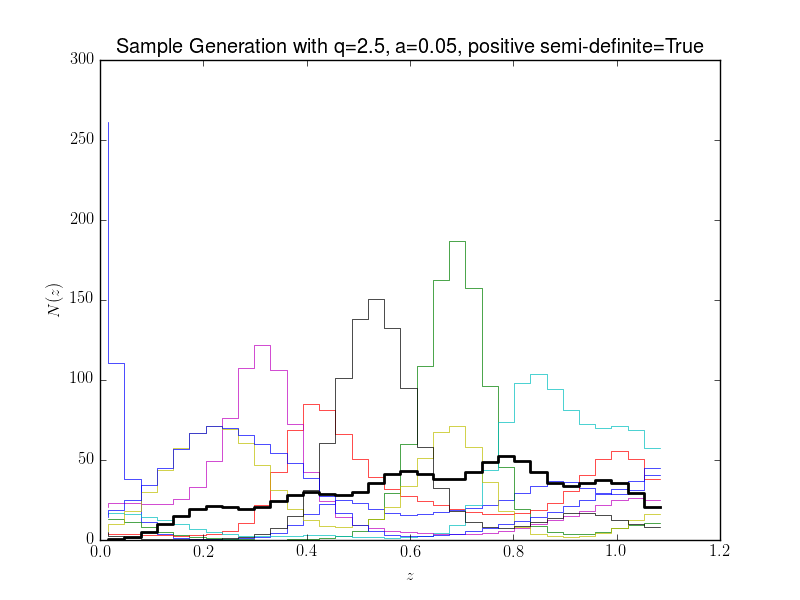
\includegraphics[scale=0.5]{samples5.png}
\caption{Several random samples of $\vec{\theta}$ from the distribution of Eq. \ref{eq:covmat} are shown here.  %As $a$ increases, more peaks are permitted and the distribution becomes less smooth.  For a set value of $q$, the amplitude of deviations from the mean decreases with $a$.
}
\end{figure}

The following pseudo-code outlines the algorithm.

\begin{enumerate}
\item \label{it:randsamp} Randomly sample Eq. \ref{eq:covmat} to generate a proposal $\ln\vec{\theta}'$.
\item Calculate the log of the numerator of the posterior as in Eq. \ref{eq:disc-post} to produce $\ln\tilde{p}(\vec{\theta}'|\textul{D})$.
\item Calculate $r=\ln\tilde{p}(\vec{\theta}'|\textul{D})-\ln\tilde{p}(\vec{\theta}|\textul{D})$.
\item If $r\geq0$, set and record $\ln\vec{\theta}=\ln\vec{\theta}'$.\\
If $r<0$, select a random number $n$ from the uniform distribution between 0 and 1.
\begin{enumerate}
\item If $n<\exp[r]$, record $\vec{\theta}_{r+1}=\vec{\theta}'$ and set $\vec{\theta}=\vec{\theta}'$
\end{enumerate}
\item Check if the threshold has been achieved; if not, return to Step \ref{it:randsamp}.
\end{enumerate}

Here, the threshold was accepting $R=100$ proposal distributions.  All accepted proposals from one instance of the code are shown in Fig. %\ref{fig:results}
.  The acceptance fraction was $\sim0.1\%$ for this and other runs.  Since 10000 iterations likely doesn't even get through the ``burn-in'' period of the algorithm, this acceptance fraction is not surprising!  If I were convinced it were otherwise valid, I would run it until some convergence criterion were achieved.  However, since that might take quite some time, I will conservatively refrain from doing so.

%\begin{figure}
%\label{fig:results}
%\includegraphics[scale=0.75]{compare-results.png}
%\caption{Accepted proposal values of $\vec{\mathcal{N}}$ are shown here, along with the true value in black.}
%\end{figure}

\section{Discussion}

It is desirable to compare this result to what would have been obtained by the method of \citet{she11}, which directly calculates the posterior for the entire dataset using the posteriors for each galaxy according to Eq. \ref{eq:sheldon}.

\begin{eqnarray}
\label{eq:sheldon}
p(B_{k}) &=& \sum_{r=1}^{R}p_{r}(B_{k}|\vec{d}_{j})
\end{eqnarray}

To do this, I calculate the posteriors $p(z|\vec{d}_{j})$ for each galaxy using Eq. \ref{eq:posts}, the product of the estimate of $\vec{\theta}$ and the likelihood for each galaxy.  This is done for all accepted values of $\vec{\theta}$.

\begin{eqnarray}
\label{eq:posts}
p_{r}(B_{k}|\vec{d}_{j}) &=& p(\vec{d}_{j}|B_{k})p(\vec{\theta}^{r}|\textul{D})
\end{eqnarray}

Fig. \ref{fig:sheldon} compares the result of summing the posteriors as in Eq. \ref{eq:sheldon} with the result of the MCMC solutions of Eq. \ref{eq:bayes}.  The method of \citet{she11} underestimates the probability of observing low redshifts.  As one would expect, the MCMC estimate irreversibly loses some substructure because of the shifting error added to the simulated data.

\begin{figure}
\label{fig:sheldon}
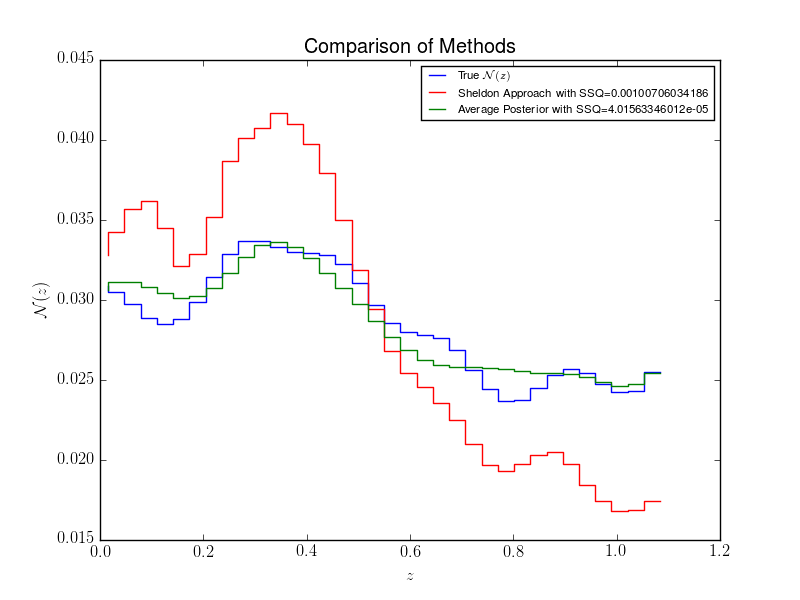
\includegraphics[scale=0.5]{compare-sheldon.png}
\caption{The result of applying Eq. \ref{eq:sheldon} is shown in red, the average accepted posterior sample from the method presented here is shown in blue, and $p(z)$ for the observable redshifts of Eq. \ref{eq:zshift} is shown in black.  The sum of squared differences between the result of each method and the true value are also shown; one can see that the \citet{she11} approach has larger errors.}
\end{figure}

%\acknowledgments

%\appendix

\begin{thebibliography}{}
\bibitem[Benitez (2000)]{ben00}
Benitez, N., ApJ 536:571-̀583, 2000 June 20
\bibitem[Cunha, et al. (2008)]{cun08}
Cunha, C.E., Lima, M., Oyaizu, H., Frieman, J., Lin, H., arxiv:0810.2991
\bibitem[Fadely, et al. (2012)]{fad12}
Fadely, R., Hogg, D.W., Willman, B., arxiv:1206.4306
\bibitem[Foreman-Mackey, Hogg, and Morton (2014)]{for14}
Foreman-Mackey, D., Hogg, D.W., and Morton, T.D., arxiv:1406.3020
\bibitem[Hogg (1999)]{hog99}
Hogg, D.W., arxiv:astro-ph/9905116
\bibitem[Hogg, et al. (2010)]{hog10}
Hogg, D.W., Myers, A.D., Bovy, J., arxiv:1008.4146
\bibitem[Hogg (2012)]{hog12}
Hogg, D.W., arxiv:1205.4446
\bibitem[Lima, et al. (2008)]{lim08}
Lima, M., Cunha, C.E., Oyaizu, H., Frieman, J., Lin, H., Sheldon, E.S., MNRAS, 390, 118
\bibitem[Marshall (2015)]{mar15}
Marshall, P., github.com/drphilmarshall/Pangloss/issues/23
\bibitem[Sheldon, et al. (2011)]{she11}
Sheldon, E.S., Cunha, C., Mandelbaum, R., Brinkmann, J., Weaver, B.A., arxiv:1109.5192

FILL IN MORE OF THESE!
\end{thebibliography}

\end{document}